\documentclass[a4paper,11pt,uplatex]{jsbook}
%\usepackage{fancyhdr}
\setlength{\footskip}{16pt}
\usepackage{amsmath}
\usepackage[dvipdfmx]{graphicx}
\usepackage[dvipdfmx]{color}
%\usepackage{pagecolor}[white]
\usepackage{amsmath,amssymb}
%\usepackage[top=3cm, bottom=3cm, left=3cm, right=3cm]{geometry}
\usepackage{braket}
\usepackage{bm}
\numberwithin{equation}{section}
\usepackage{mathrsfs}
\usepackage{siunitx}
\usepackage{physics}
\usepackage[dvipdfmx]{graphicx}
\usepackage[compat=1.1.0]{tikz-feynhand}
\usepackage{caption}
\usepackage{subcaption}
%\usepackage{cleveref}
\usepackage{float}
\usepackage{multicol}
\setlength{\columnsep}{15mm}
%\usepackage[style=phys,articletitle=false,biblabel=brackets,chaptertitle=false,pageranges=false]{biblatex}
%\usepackage[style=phys]{biblatex}
\usepackage[dvipdfmx]{hyperref}
\usepackage{url}
\usepackage{pxjahyper}
\usepackage{bookmark}
%\usepackage[backref]{hyperref}
\setcounter{tocdepth}{3}
\setlength{\parindent}{2em}
\def\vector#1{\mbox{\boldmath $#1$}}
\def\slash#1{\not\!#1}
\def\slashb#1{\not\!\!#1}
\def\delsla{\not\!\partial}
%\usepackage[dvipdfmx]{xcolor}


\hypersetup{
 setpagesize=false,
 bookmarksnumbered=true,%
 bookmarksopen=true,%
 colorlinks=true,%
 linkcolor=black,
 citecolor=red,
 urlcolor=black,
}
%backreferenceのカスタマイズ. "Back to p.3"のように表示する.
%\renewcommand*{\backref}[1]{(p.#1へ戻る)}
%\newcommand{\backtoc}{\hyperlink{toc}{[目次へ]}}
\newcommand{\backtoc}{\texorpdfstring{\protect\hyperlink{toc}{\hspace{5pt} \scriptsize [目次へ]}}{}}
\newcommand{\mychapter}[1]{\chapter[#1]{#1\backtoc}}
\newcommand{\mysection}[1]{\section[#1]{#1\backtoc}}
\newcommand{\mysubsection}[1]{\subsection[#1]{#1\backtoc}}

% 数式
%\usepackage{amsmath,amsfonts}
%\usepackage{bm}
%\usepackage{physics}
% 画像
%\usepackage[dvipdfmx]{graphicx}
%\usepackage[dvipdfmx,colorlinks=true,linkcolor=blue]{hyperref}
%\usepackage{pxjahyper}

\begin{document}

\chapter{データ解析と結果}
この章ではデータ解析の手順と結果について述べる。

単独アンジュレータのデータおよびエネルギー測定用の2台のアンジュレータのデータの2つのデータセットがある。
画像処理までの手順は共通であるのでまずは画像処理について述べる。
続いて単独アンジュレータのデータの解析結果を述べる。
最後に2台のアンジュレータのデータの解析結果について述べる。\\
なおエネルギー測定のデータセットは以下のように構成されている。
\begin{itemize}
  \item 水銀灯の波長較正データ1枚
  \item アンジュレータの位置データ 166個の値
  \item 干渉光の画像データ 166 position $\times$ 4 画像 = 664枚
\end{itemize}
これを反映し、エネルギーデータ解析の手順は以下のようになる。
\begin{enumerate}
  \item 波長較正 波長 - px直線を求める
  \item 画像の統合 664枚-> 166枚の二次元データ
  \item 較正波長でのデータの切り出し 166枚の二次元データ-> 166成分の1次元データ
  \item モデル関数によるフィッティング
\end{enumerate}

\section{画像処理}
\noindent \textbf{\underline{解析}}\par
まず電子ビームを入射していない状態の画像を取得し、これを背景画像とする。露光時間10 秒で10枚の画像を連続で取得し、背景画像とした。\\
各runでは、各ポジションで4枚の画像が取得される。
これらの4枚の画像について、各ピクセルごとに平均値を取り、その値をピクセルの代表値とする。
またピクセルの誤差は4枚のピクセルの標準偏差とする。\\
予想される回折パターンの性質を考えると、隣り合うピクセル同士の発光量の差は周囲の上下左右のピクセルに対して極端に発光量が多いピクセルはノイズであると判断してマスクし、フィッティングの対象に含まない。

\noindent \textbf{\underline{結果}}\par
あるピクセルにおける、4枚の画像の平均値と標準偏差の関係を図\ref{pixel}に示す。
\begin{figure}[h]
  \centering
  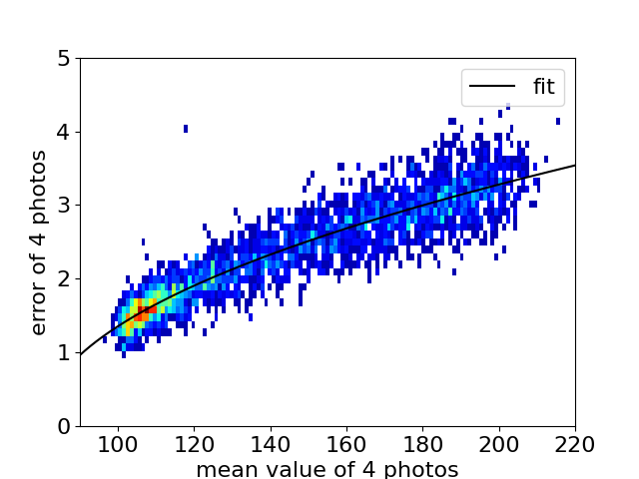
\includegraphics[width=0.8\linewidth]{image/4-pixel.png}
  \caption{ピクセルの平均値と標準偏差の関係}\label{pixel}
\end{figure}
ピクセルの発光量はポアソン分布に従うことから、標準偏差は平均値の平方根に比例すると考えられる。
オフセットを考慮してフィッティングした結果、平均値と標準偏差の関係は
\begin{eqnarray}
  \text{std} = 0.298(4) \sqrt{\text{mean} - 79.2(1.6) } 
\end{eqnarray}
となった。

背景画像の結果を示す。平均してピクセル値が100 程度、標準誤差は5程度となった。

全てのピクセルの平均値と標準偏差の関係を示す。

周囲のピクセルと比較した超過値の分布を示す。閾値として今回は40を設定した。超過値が40を超えるピクセルはノイズピクセルとして除去した。
ノイズピクセルと判定されたピクセルの割合は平均して??\%であった。
また、ピクセルが異常を起こし、常にノイズピクセルとして判定される割合は??\%程度だったのに対し、放射線など偶発的にノイズが乗るピクセルは??\%程度であった。
\subsection{平滑化}
画像の平滑化が必要な場合には、波長方向にのみ行う。同様にノイズピクセルをマスクしたうえで、マスクされなかったピクセルの平均値と標準偏差を計算し、ピクセルの誤差は標準偏差を計算に用いたピクセル数の平方根で割った値(標準誤差)とする。

\section{波長較正}
\noindent \textbf{\underline{解析}}\par
水銀灯の404.656 nmおよび407.781 nmの輝線スペクトルをガウシアンでフィットし、ピーク中心の位置を求める。
2本の輝線から、波長 - pxの線形性を仮定し、画像全体の波長 - px直線を求める。
ピークの中心決定精度から波長較正の精度を求める。

\noindent \textbf{\underline{結果}}\par
水銀灯の波長較正で得られた画像の例を示す。
\begin{figure}
  \centering
  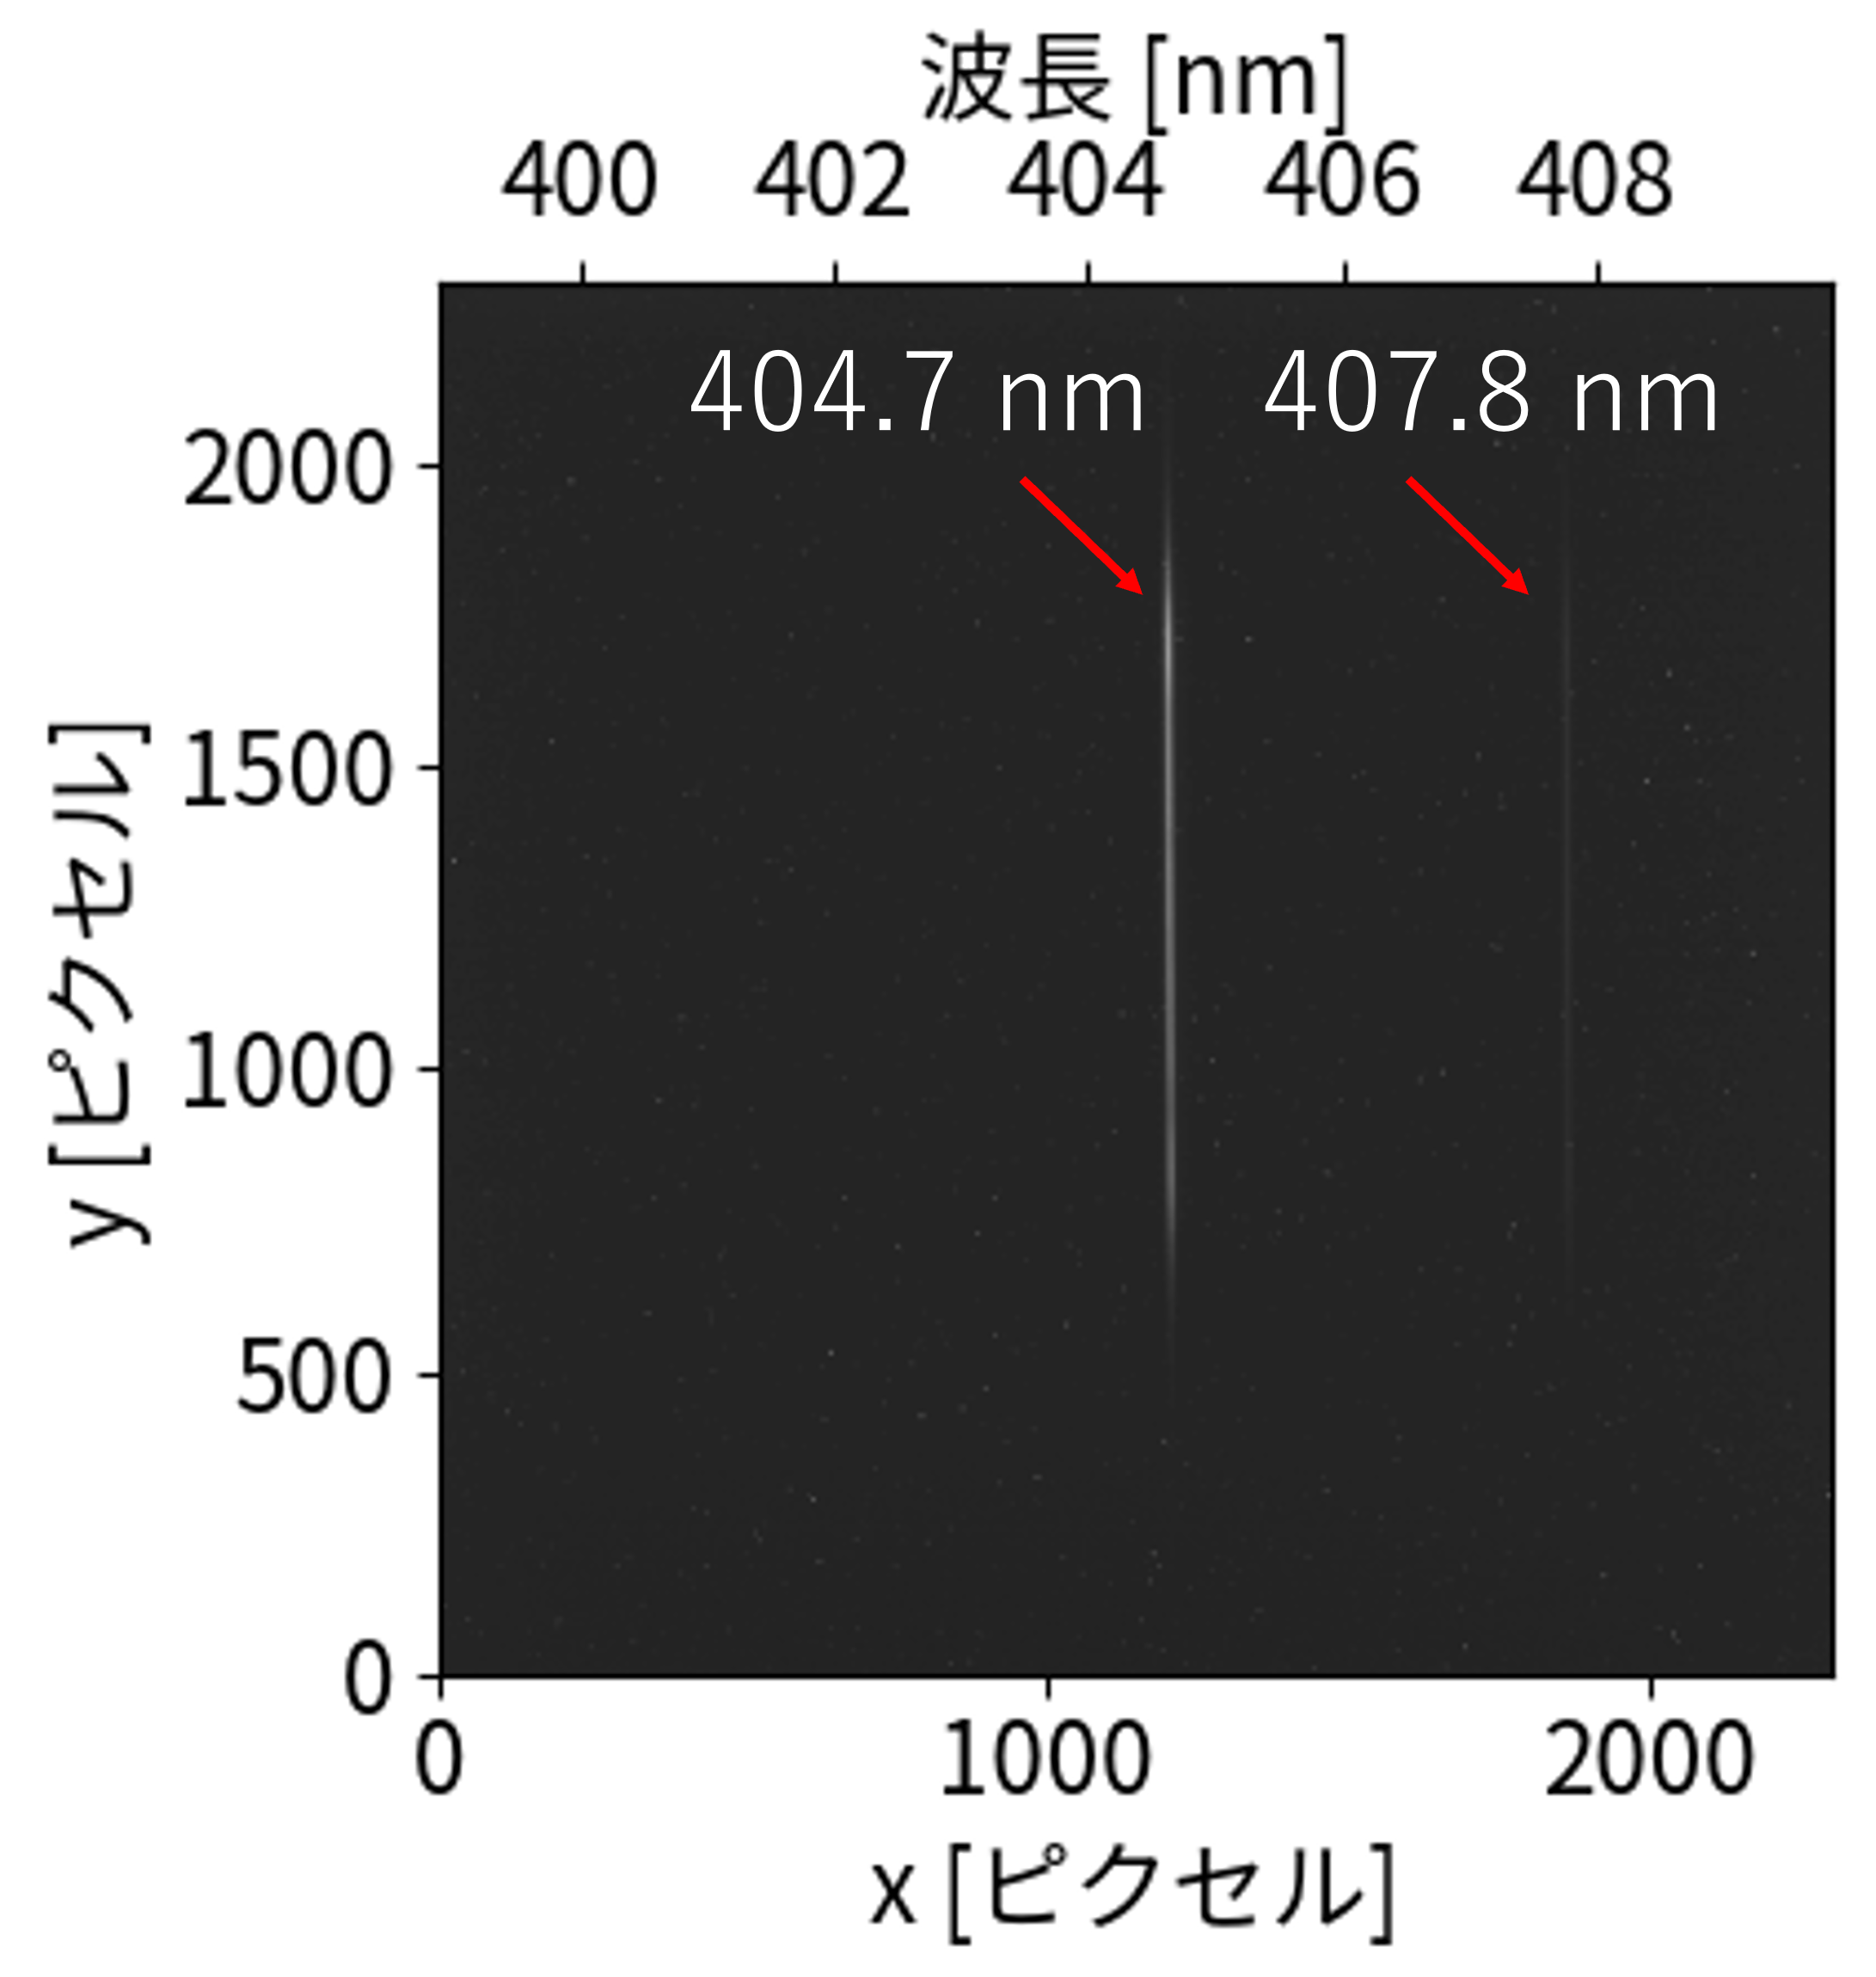
\includegraphics[width=0.8\linewidth]{image/4-mercury.png}
  \caption{水銀灯の波長較正}
\end{figure}
縦軸方向に50 pxのカットをかけてガウシアンによるフィッティングを行った結果を示す。
\begin{figure}
  \centering
  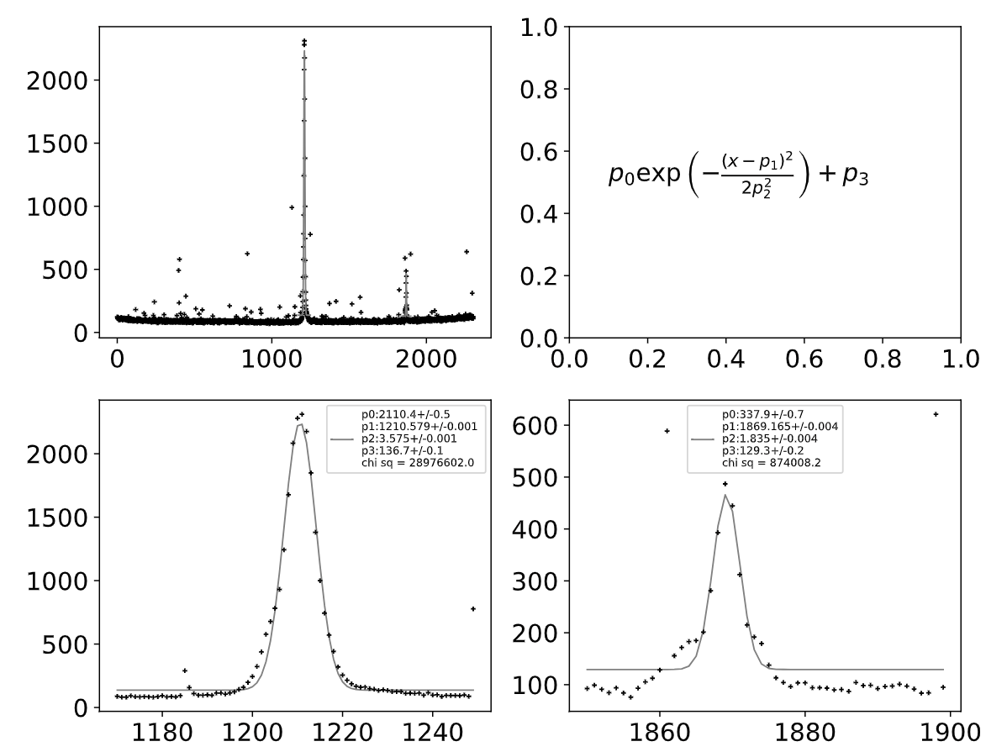
\includegraphics[width=0.8\linewidth]{image/4-mercuryfit.png}
  \caption{水銀灯の波長較正}
\end{figure}

\section{モデル関数によるフィッティング}
\noindent \textbf{\underline{解析}}\par
この節では、単独アンジュレータのデータおよび2台のアンジュレータのデータ両方の解析に用いるモデル関数について述べる。モデル関数は、エネルギーを含む各種パラメータとアンジュレータの位置を入力として、回折パターンの形状をカメラのy座標の関数として出力する関数である。
\subsection{1電子放射光関数}
アンジュレータ放射光の振幅は放射角の関数として以下のように計算できることが知られている。
また放射光の位相は球面波を仮定する。

\subsection{フレネル回折}
放射光関数で計算されたスリットにおける光波($U(x)$)から、カメラにおける回折光を計算する。フレネル近似を用いて計算を行う。

\subsubsection{数値計算上の計算手法}
数値計算を実行する上では数値積分の手法では、伝搬後のN次元の配列が伝搬前のN次元配列全ての積分を用いて計算されるため計算量は$\text{N}^2$となる。
このような計算コストの高い計算を避けるために、高速フーリエ変換を用いた計算が一般に用いられている。
式(\ref{レイリーゾンマーフェルト近似})を再度$x,y,x_0,y_0$で書き直すと
\begin{eqnarray}
  \text{U}(x_0,y_0) \sim \frac{1}{2i\lambda zs}\int_S \text{U}(x,y) \exp( ik \sqrt{z^2 + (x-x_0)^2 + (y-y_0)^2}) dxdy
\end{eqnarray}
これはカーネル関数$f(x,y) = \sqrt{z^2 +x^2 + y^2}$であるような畳み込みの形で書ける。
\begin{eqnarray}
  U(x_0,y_0) \sim (\text{U} * f)(x,y)
\end{eqnarray}
畳み込みはフーリエ変換を用いることで
\begin{eqnarray}
  (U*f)(x,y) = \mathcal{F}^{-1}(\mathcal{F}(U) \times \mathcal{F}(f)) \label{convolution}
\end{eqnarray}
と表せる。ここで$\mathcal{F}$はフーリエ変換を表す。これは以下のように示すことができる。
\begin{eqnarray}
  (U*f)(x) = \int_{-\infty}^{\infty} U(t)f(x-t)dt
\end{eqnarray}
これをフーリエ変換したものは、
\begin{eqnarray}
  \mathcal{F}(U*f)(k) = \int_{-\infty}^{\infty} \int_{-\infty}^{\infty} U(t)f(x-t)dt \exp(-ikx)dx
\end{eqnarray}
積分の順序を交換して$x-t = y$とおくと、
\begin{eqnarray}
  \mathcal{F}(U*f)(k) &=& \int_{-\infty}^{\infty} U(t) \exp(-ikt)dt \int_{-\infty}^{\infty} f(y) \exp(-iky)dy\\
  &=& \mathcal{F}(U) \times \mathcal{F}(f)
\end{eqnarray}
したがって\ref{convolution}が示される。

フーリエ変換による計算では、周波数空間のあらわす光波は計算空間と同じ大きさの周期的な光波として表現される。そのため、そのまま逆変換を行うと隣り合う計算空間の光波が干渉してしまう。これを防ぐために、計算空間の端を0で埋め、計算空間を拡大するゼロパディングを行う。

\subsection{電子ビームサイズ}
1電子の放射光であると仮定していた放射光関数は、電子ビームサイズを考慮すると、異なる電子からの放射光関数の重ね合わせとして表現できると考えられる。
y軸方向のビームサイズを$\sigma_y$として、ガウス上の広がりを考慮し、放射光関数を畳みこむ。
これにより1電子放射光関数から得られる回折パターンはぼやける。
\subsection{光学系}
回折格子によって分光された光はレンズによってカメラで収束する。スリットの形状および回折格子はx方向にも幅を持つが、計算時間の都合上y軸方向のみの1次元の計算を行う。
1次元の回折と2次元の回折の結果はほとんど変わらないことが確認されている。
\subsection{パラメータ}
求める関数系は放射光関数と光学系関数からなる。
パラメータの定義を以下に示す。
\begin{table}[h]
\centering
\begin{tabular}{c|c}
  $\gamma$ & 電子ビームエネルギーのローレンツ因子 \\
  $\text{K}$ & アンジュレータのK値 \\
  $\text{z(U2-slit)}$ & 下流アンジュレータ-スリット間の距離 \\
  $\text{z(slit-camera)}$ & スリット-カメラ間の距離 \\
  $\text{w(slit)}$ & スリットの鉛直方向の長さ \\
  $\text{y(beam)}$ & カメラに対するビーム中心のy座標 \\
  $\text{y(slit)}$ & カメラに対するスリット中心のy座標 \\
  $\delta \phi$ & 上流と下流のアンジュレータの位相のずれ\\
\end{tabular}
\end{table}

\subsection{パラメータ較正}
単独アンジュレータのデータを解析し、z(U2- slit),z(slit-camera),w(slit)の最適値を求める。
2台のアンジュレータのデータではこれらのパラメータを固定してフィッティングを行う。ただし系統誤差を見積もるために、パラメータを変化させた場合のフィッティングも行う。\\
また、アンジュレータが下流に移動することによる光量の変化をampl パラメータのd依存性に押し込む。この依存性から、上流アンジュレータと下流アンジュレータの寄与の係数も決定できる。
\section{単独アンジュレータの解析}
\noindent \textbf{\underline{解析}}\par
パラメータ較正を目的とした単独アンジュレータのデータの解析を述べる。
下流アンジュレータのみの磁場によって得られるデータから、放射光関数の位置依存性の情報が抽出できる。
理想的な条件では、アンジュレータが下流に移動すると以下のような変化が見られると考えられる。
\begin{itemize}
  \item アクセプタンスの増加による振幅の増加
  \item 光学的な位置関係の変化による回折パターンの形状の変化
\end{itemize}

振幅の上昇と回折パターンの形状の変化から、距離のパラメータ z(U2-slit),z(slit-cam),w(slits)の最適値を求めることができる。
z(U2-slit),z(slit-cam),w(slit)を固定してフィッティングを行い、適合度がもっとも良いパラメータの組を最適な値として定義する。
\noindent \textbf{\underline{結果}}\par

\subsubsection{波長依存性}
波長依存性があり長波長側の光量が大きい傾向がある。
この傾向は線形の依存性が仮定できる。\\
\subsubsection{位置依存性}
アンジュレータの位置に対する依存性があり、アンジュレータが下流に移動するにつれて3つの傾向が見られる。
\begin{itemize}
  \item 回折パターンの振幅が上昇する
  \item 回折パターンの形状が変化する
  \item 回折パターンの振幅が周期的に小さく変動する
\end{itemize}
振幅の上昇と周期的な変動は放射角に対して一様ではない。特にピーク位置を抽出して振幅の変化をみると、
ピークごとに異なる上昇率が見られる。これはアンジュレータ位置に対して回折パターンの形状も変化することが影響していると推定できる。
一方で回折パターンの振幅はどのピクセルにおいてもほぼ一定であり、その振幅は電子ビームエネルギー210 MeVの振幅と対応している。
偏極電磁石による一定位相の放射との干渉が見えていると考えることができる。
実際に一定位相の偏極電磁石放射を仮定してシミュレーションした結果によれば、振幅の傾向は一致する。\\
\subsubsection{放射光および光学系パラメータ}
回折パターンの形状を決定するパラメータはアンジュレータ - スリット間距離、スリット - カメラ間距離、スリット幅の3つである。
これに加えて放射光関数の情報も形状を決定する。放射光関数の形状は理論式を仮定し、z(U2-slit)、z(slit-cam)、w(slit)の3つのパラメータの最適値を決定する。\\
アンジュレータと光学系の距離に依存して光量が変化する。立体角を考えるとこの光量はスリットからの距離rに対して$\frac{1}{r^2}$に比例すると考えられる。
また距離によって振幅が周期的に変動する効果は、偏極電磁石による放射だと考えることができる。
このような仮定に基づいて単独アンジュレータのデータをフィットした。\\
またパラメータを固定した時の適合度の比較の結果を示す。
これらの結果からパラメータの値を??と決定した。
またパラメータの決定精度は??である。

\section{2台のアンジュレータの解析}
\noindent \textbf{\underline{解析}}\par
パラメータ較正によって決定したパラメータを用いて2台のアンジュレータのデータを解析する。動かすパラメータは以下の通りである。
\begin{table}[h]
\centering
\begin{tabular}{cc}
  $\gamma$ & 電子ビームエネルギーのローレンツ因子 \\
  y(beam) & カメラに対するビーム中心のy座標 \\
  y(slit) & カメラに対するスリット中心のy座標 \\
  $\delta \phi$ & 上流と下流のアンジュレータの位相のずれ\\
  ampl & 振幅
\end{tabular}
\end{table}
これらのパラメータを動かしてモデル関数によるデータのフィッティングを行う。
フィッティングは既約カイ二乗値による最小二乗法を用いる。
またpythonのminuitパッケージを用いてフィッティングを行う。\\
フィッティングで得られた$\gamma$の値から電子ビームエネルギーを求める。

\noindent \textbf{\underline{結果}}\par
2台のアンジュレータで得られる画像の例を示す。アンジュレータの位置によって回折パターンの形状が変化することがわかる。波長によって振動の初期位相が違うため、強弱が短波長側に移動していくように見える。

較正波長404.65 nm、y軸方向の中心のピクセルの周期的変動を、アンジュレータの位置に対してプロットした結果の例を示す。周期的変動がみられることがわかる。
\begin{figure}
  \centering
  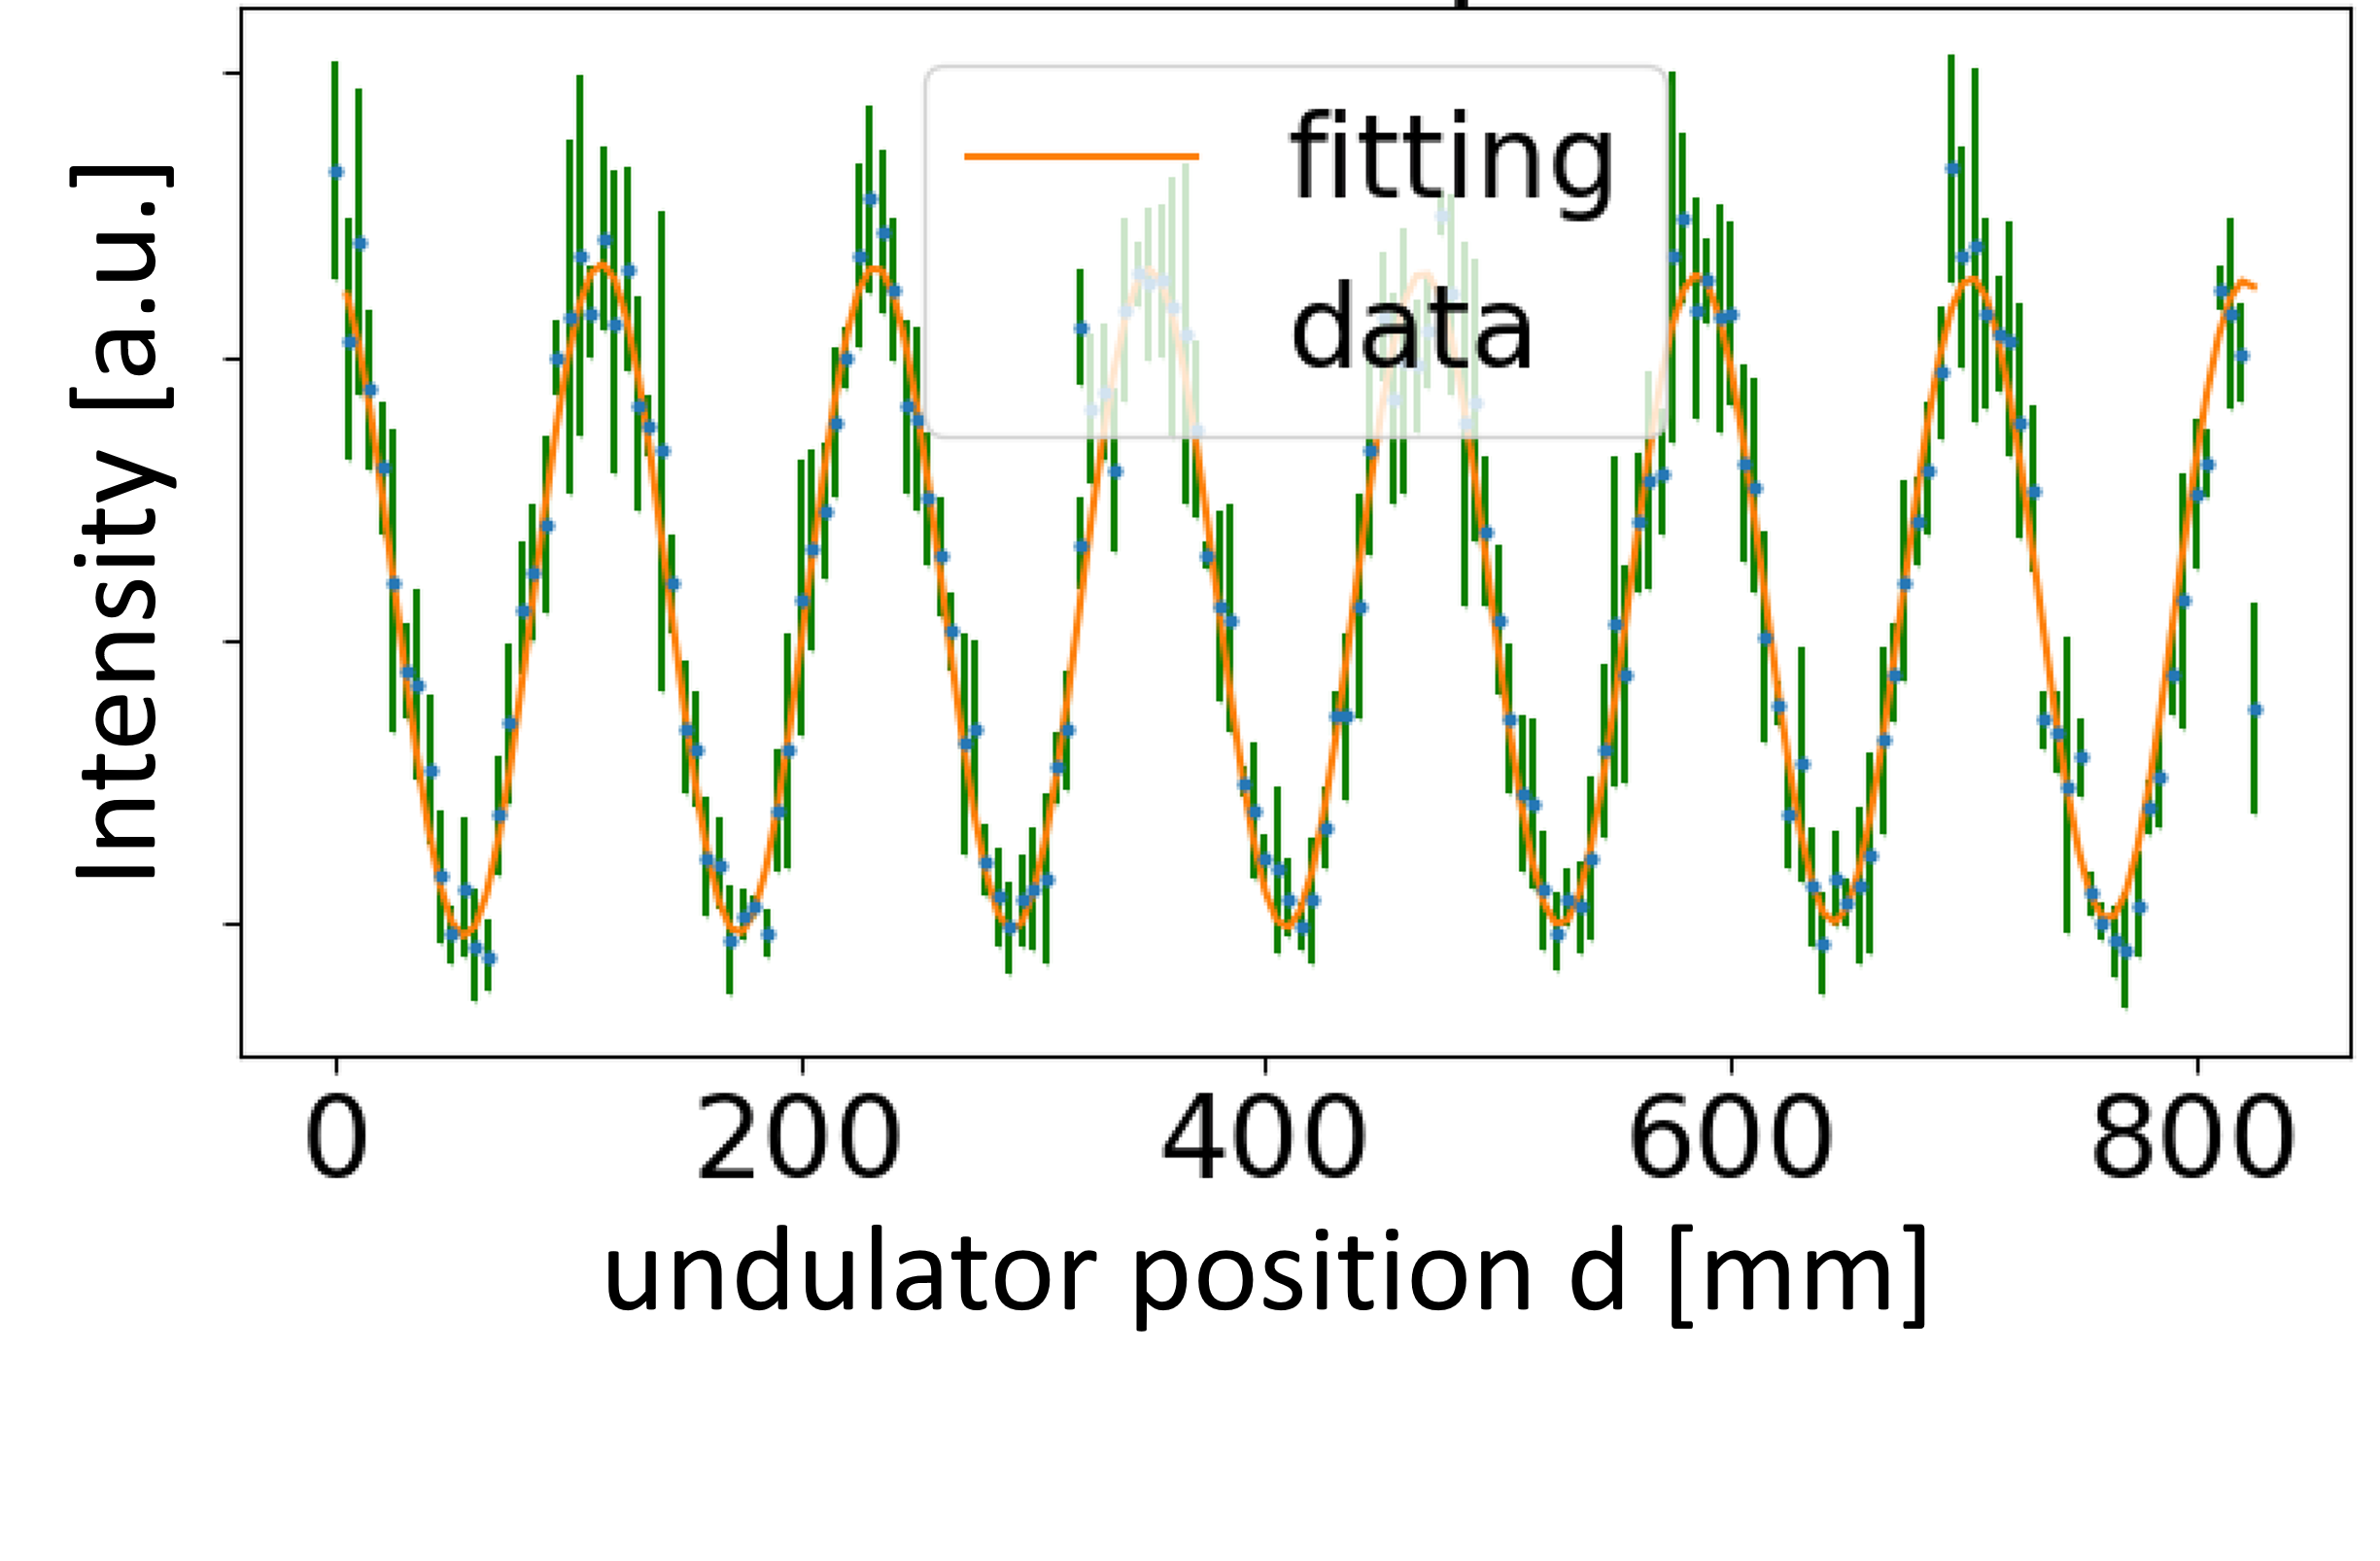
\includegraphics[width=0.8\linewidth]{image/4-oscillation.png}
  \caption{アンジュレータ位置に対する振幅の変化}
\end{figure}

\section{統計誤差の見積もり}
\noindent \textbf{\underline{解析}}\par
統計誤差の見積もりはブートストラップ法によって行う。
ブートストラップ法はデータから復元抽出を行い、その復元抽出データから統計量を計算することで統計量の分布を推定する手法である。
下流アンジュレータの位置に関してランダムに復元抽出を複数回行い、抽出されたデータの集合に対してフィッティングを行う。得られたパラメータの分布から統計誤差を見積もる。

また各パラメータ同士の相関もブートストラップ法の復元抽出データから求めることができる。
理想的には全てのパラメータ同士が相関を持たない。

\noindent \textbf{\underline{結果}}\par
ブートストラップ法による統計誤差の見積もりの結果を示す。100個の異なる復元抽出データから得られる
$\gamma$の分布を示す。この分布から求めた$\gamma$の平均値と標準偏差は??である。
\section{系統誤差の見積もり}
波長依存性と位置依存性による系統誤差が主要な誤差要因と考えられる。
\subsubsection{波長依存性}
\noindent \textbf{\underline{解析}}\par
較正波長(404.65 nm)におけるエネルギー測定の結果に加えて、同じモデル関数を用いて異なる波長でのデータからエネルギーを求める。
異なる波長に対するエネルギーの分布から、モデル関数や装置のもつ波長依存性による系統誤差を見積もる。

\noindent \textbf{\underline{結果}}\par
横軸を波長に、縦軸をその波長における$\gamma$の推定値としたグラフを図\ref{wldep}に示す。
\begin{figure}[h]
  \centering
  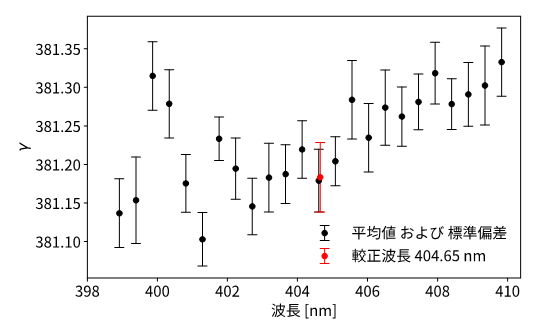
\includegraphics[width=0.8\linewidth]{image/4-wldep.png}
  \caption{エネルギーの推定値の位置依存性}\label{wldep}
\end{figure}

また、アクセプタンス全体における$\gamma$の分布から波長依存性による系統誤差は??と見積もられた。
\subsubsection{位置依存性}
\noindent \textbf{\underline{解析}}\par
アンジュレータの位置によるエネルギーの推定値の違いを見積もる。
具体的には、アンジュレータの位置を4つの区間に分割し、各区間でエネルギーを求める。アンジュレータ位置に対する放射光関数の補正がどの程度の影響を持つかを見積もる。

\noindent \textbf{\underline{結果}}\par
横軸を4分割の区間のインデックス、縦軸を各区間で得られた$\gamma$の推定値としたグラフを図\ref{posdep}に示す。
\begin{figure}[h]
  \centering
  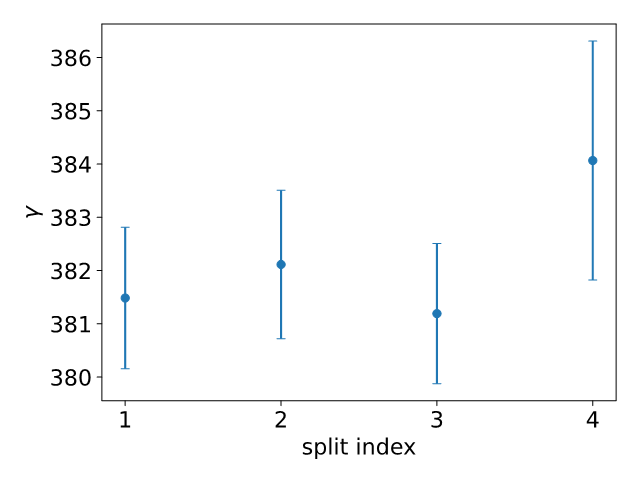
\includegraphics[width=0.8\linewidth]{image/4-posdep.png}
  \caption[アンジュレータ位置に対するエネルギーの推定値]{アンジュレータ位置に対するエネルギーの推定値。split index 1がもっとも上流であり、アンジュレータの可動範囲の最上流を0 mm としたときに
  split index 1は 0 mm から205 mm、split index 2は205 mmから410 mm、split index 3は415 mmから620 mm、split index 4は620 mmから825 mmの範囲を示す。}\label{posdep}
\end{figure}

\subsubsection{エネルギー依存性}
180、195、210 MeVの3つのエネルギーの結果を表に示す。

\end{document}